% Scoring, Not Solving --- a verification oracle for materials physics.
% Rendered draft of the slide-deck outline (companion: 2026-06-25-physics-as-a-cs-oracle.md).
% Presentation artifact; NOT part of the lint-enforced atomic tree.
%
% Build:  pdflatex 2026-06-25-physics-as-a-cs-oracle.tex   (run twice)
% Engine: pdflatex (portable; metropolis falls back to Latin Modern, no Fira needed).
%
\documentclass[aspectratio=169,10pt]{beamer}
\usetheme{metropolis}
\metroset{block=fill, sectionpage=progressbar}

\usepackage[T1]{fontenc}
\usepackage[utf8]{inputenc}
\usepackage{textcomp}
\usepackage{amsmath,amssymb}
\usepackage{booktabs}
\usepackage{tikz}
\usepackage{tikz-cd}
\usetikzlibrary{automata, positioning, arrows.meta, fit, backgrounds, calc, shapes.geometric}

% --- node-kind colours for the typed DAG ---
\definecolor{kInput}{HTML}{1B998B}
\definecolor{kFormula}{HTML}{2E86AB}
\definecolor{kMethod}{HTML}{E08E0B}
\definecolor{kResid}{HTML}{8E4585}

\newcommand{\code}[1]{\texttt{#1}}
\newcommand{\cz}[1]{({\scriptsize\color{gray}#1})}     % inline source pointer
\setbeamertemplate{frame numbering}[fraction]

\begin{document}

% ===================================================================== Title
{\setbeamertemplate{frame numbering}[none]
\begin{frame}[plain]
  \centering
  \vspace{0.6cm}
  {\Huge\bfseries Scoring, Not Solving}\\[0.5em]
  {\large A verification oracle for materials physics}\\[1.3em]
  \rule{0.55\textwidth}{0.4pt}\\[1.1em]
  {\itshape It is harder to solve a problem than to verify a solution ---\\
   so verification is what has been built.}\\[1.6em]
  {\footnotesize Application: durable ultra-wide-bandgap devices for harsh operating conditions.}\\[2.2em]
  {\normalsize Javier Flores \quad\textperiodcentered\quad 2026-06-25}
\end{frame}}

% ===================================================================== Sec 1
\section{The asymmetry}

\begin{frame}{The asymmetry}
  \framesubtitle{Finding an answer is hard. Checking an answer is easy.}
  \begin{itemize}
    \item The defining property of \textbf{NP}: a \emph{certificate} (a witness) is checkable in
      polynomial time even when finding it is exponentially hard. Sudoku, factoring,
      satisfiability --- hard to solve, trivial to check.
    \item \code{/physics} lives on the \alert{cheap side of that gap on purpose}: it never
      searches for the state; it grades a state it is handed.
    \item The whole system is engineered to make \emph{checking} fast, exhaustive, and
      trustworthy.
  \end{itemize}
  \note{The organizing idea; flag that it returns five times. Everything downstream (compiler,
  types, AD) is in service of cheap, trustworthy checking.}
\end{frame}

\begin{frame}{A pure oracle}
  \framesubtitle{Input: a candidate state. Output: how far it violates physics law, plus a certificate.}
  \begin{center}
  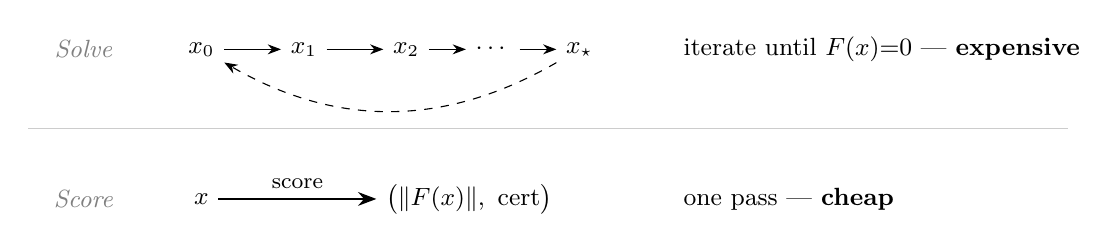
\begin{tikzpicture}[>=Stealth, font=\small]
    \node[gray] at (-1.5,0) {\itshape Solve};
    \node (s0) at (0,0) {$x_0$};
    \node (s1) at (1.3,0) {$x_1$};
    \node (s2) at (2.6,0) {$x_2$};
    \node (sd) at (3.7,0) {$\cdots$};
    \node (ss) at (4.8,0) {$x_\star$};
    \foreach \a/\b in {s0/s1,s1/s2,s2/sd,sd/ss} \draw[->] (\a)--(\b);
    \draw[->,dashed] (ss) to[out=-150,in=-30] (s0);
    \node[anchor=west] at (6.0,0) {iterate until $F(x){=}0$ --- \textbf{expensive}};
    \draw[gray!40] (-2.2,-1.0) -- (11.0,-1.0);
    \node[gray] at (-1.5,-1.9) {\itshape Score};
    \node (in)  at (0,-1.9) {$x$};
    \node (out) at (3.4,-1.9) {$\bigl(\lVert F(x)\rVert,\ \text{cert}\bigr)$};
    \draw[->,thick] (in) -- node[above]{\footnotesize score} (out);
    \node[anchor=west] at (6.0,-1.9) {one pass --- \textbf{cheap}};
  \end{tikzpicture}
  \end{center}
  \begin{itemize}\small
    \item \code{/physics} is a pure oracle: it owns no training loop and no sample-selection
      logic \cz{\code{arch-01-purpose} \S72--75}.
    \item The scoring principle holds at every length-and-time scale --- femtoseconds to years,
      atom to device \cz{\code{arch-21-multiscale-state} \S87--88}.
  \end{itemize}
  \note{The candidate state comes from a learned model (the neural operator) --- another talk.
  Here the operator is just whoever supplies an x. Keep the focus on the oracle's one job.}
\end{frame}

\begin{frame}{The cost ladder}
  \framesubtitle{Checking runs in microseconds where solving runs in minutes.}
  \footnotesize
  \setlength{\tabcolsep}{5pt}
  \begin{center}
  \begin{tabular}{@{}llll@{}}
    \toprule
    Tier & Budget & Cadence & Shape of the work\\
    \midrule
    \textbf{T0} & $\leq 10\,\mu$s, closed-form & every gradient step & a few arithmetic ops\\
    \textbf{T1} & $\leq 10\,$ms, small lin.\ alg.\ / 1-D quad. & per batch (sampled) & a small dense solve\\
    \textbf{T2} & $\leq 10\,$s, bounded integral on a grid & per epoch (cached) & a sweep over a fixed mesh\\
    \textbf{T3} & $\leq 10\,$min, iterative solve / PDE & calibration only & a fixed-point loop to convergence\\
    \bottomrule
  \end{tabular}
  \end{center}
  \vspace{0.6em}
  \normalsize
  The corresponding \emph{solve} --- a full iterative loop from scratch --- is the \textbf{T3}
  rung, minutes. The oracle keeps scoring on the \textbf{T0/T1} rungs, ``fast by construction''
  \cz{\code{arch-07-pipeline} \S28--32}.
  \note{The thesis made quantitative. The four-orders-of-magnitude gap between check (microseconds)
  and solve (minutes) is the entire reason a learning loop is feasible: millions of candidates can
  be graded.}
\end{frame}

\begin{frame}{The certificate}
  \framesubtitle{Every score ships with a small, independently checkable proof object.}
  \begin{columns}[T]
    \column{0.62\textwidth}
    \begin{itemize}\small
      \item ``an inert s-expression carrying scalar verdicts plus numeric witnesses for
        failures'' \cz{\code{arch-12-cert} \S19--22} --- an NP-style certificate: cheap to check,
        carries its own evidence.
      \item A failure carries a \textbf{witness} --- the exact offending input, e.g.\ the pair of
        values that broke a consistency rule \cz{\S109--119}.
      \item Ten obligations: symmetry, bounds, analytic limits, reference battery, conservation,
        consistency, bulk--boundary, versioning, surrogate validity, adjoint existence
        \cz{\S24--40}.
    \end{itemize}
    \column{0.38\textwidth}
    \begin{center}
    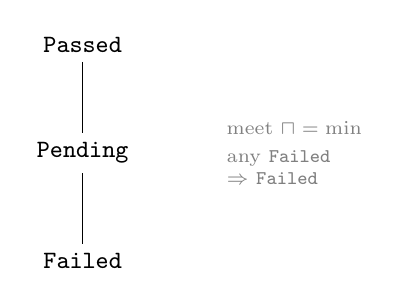
\begin{tikzpicture}[>=Stealth, node distance=9mm, font=\small]
      \node (p) {\code{Passed}};
      \node (q) [below=of p] {\code{Pending}};
      \node (f) [below=of q] {\code{Failed}};
      \draw (p)--(q); \draw (q)--(f);
      \node[right=10mm of q, align=left, font=\scriptsize, color=gray]
        {meet $\sqcap=\min$\\[2pt] any \code{Failed}\\ $\Rightarrow$ \code{Failed}};
    \end{tikzpicture}\\[0.4em]
    {\scriptsize Verdicts combine by a semilattice meet \cz{\code{impl-07} \S56--60}.}
    \end{center}
  \end{columns}
  \note{Emphasize independently checkable: the cert is inert data, so an auditor later can
  re-verify a result without re-running the oracle --- the claim comes with its receipt.}
\end{frame}

% ===================================================================== Sec 2
\section{Physics as a language}

\begin{frame}{The alphabet and grammar}
  \framesubtitle{The physics being scored is a closed formal language.}
  \begin{columns}[T]
    \column{0.5\textwidth}
    \begin{itemize}
      \item 12 computational \textbf{methods} (+3 sub)
      \item 20 abstract-property \textbf{templates}
      \item 125 named \textbf{formulas} (+2 markers)
    \end{itemize}
    \column{0.5\textwidth}
    \begin{itemize}
      \item 11 observable \textbf{bundles}
      \item 19 \textbf{residual categories}
      \item 10 \textbf{cert obligations}, 4 \textbf{typeclasses}
    \end{itemize}
  \end{columns}
  \vspace{0.8em}
  \begin{itemize}
    \item ``instances are programs in this vocabulary'' \cz{\code{arch-09-vocabularies} \S9.1}.
    \item A finite, decidable grammar makes the set of well-formed questions \textbf{enumerable
      and exhaustive} --- ``there should be no more questions one can ask.''
  \end{itemize}
  \note{An open-ended pile of formulas can never be complete. Closing the set and making
  composition the only growth mechanism turns exhaustiveness into a provable property.}
\end{frame}

\begin{frame}{The abstract syntax tree}
  \framesubtitle{A composed physics problem is a typed, content-addressed DAG.}
  \begin{columns}[T]
    \column{0.5\textwidth}
    \begin{itemize}\small
      \item The \code{PhysicsGraph}: ``a typed, hash-consed, content-addressed directed acyclic
        graph'' \cz{\code{arch-06-physics-graph}}.
      \item Three node kinds --- the grammar's terminals:
        \code{Input}, \code{FormulaApply}, \code{MethodInvoke} \cz{\S6.2}.
      \item The 125 formulas and 12 methods are \textbf{typing rules} for these nodes \cz{\S6.5}.
      \item Composing observables \emph{is} composing subgraphs --- a new observable is a new
        sentence, not new code.
    \end{itemize}
    \column{0.5\textwidth}
    \begin{center}
    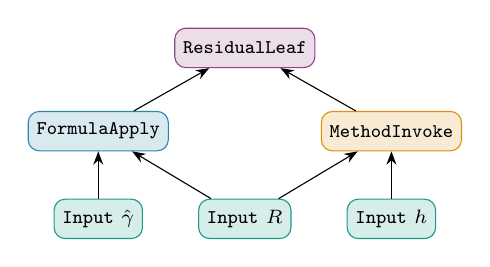
\begin{tikzpicture}[>=Stealth, font=\scriptsize, node distance=6mm and 7mm,
      every node/.style={rounded corners, draw, minimum height=5mm, inner sep=3pt}]
      \node[fill=kInput!18, draw=kInput] (i1) {\code{Input} $\hat\gamma$};
      \node[fill=kInput!18, draw=kInput, right=of i1] (i2) {\code{Input} $R$};
      \node[fill=kInput!18, draw=kInput, right=of i2] (i3) {\code{Input} $h$};
      \node[fill=kFormula!18, draw=kFormula, above=of i1] (f1) {\code{FormulaApply}};
      \node[fill=kMethod!18, draw=kMethod, above=of i3] (m1) {\code{MethodInvoke}};
      \node[fill=kResid!18, draw=kResid, above=8mm of $(f1)!0.5!(m1)$] (r) {\code{ResidualLeaf}};
      \draw[->] (i1)--(f1); \draw[->] (i2)--(f1);
      \draw[->] (i2)--(m1); \draw[->] (i3)--(m1);
      \draw[->] (f1)--(r);  \draw[->] (m1)--(r);
    \end{tikzpicture}\\[0.5em]
    {\scriptsize Shared child $R$ feeds two parents: hash-consing makes it a DAG, not a tree.}
    \end{center}
  \end{columns}
  \note{Source code to AST to typed IR --- a physics composition takes the same path. This reframes
  add a property from a coding task to a parsing task, which unlocks the compiler next.}
\end{frame}

% ===================================================================== Sec 3
\section{The compiler}

\begin{frame}{\code{/physics} is a compiler}
  \framesubtitle{It parses a physics problem and compiles it to a numerical kernel.}
  \begin{center}
  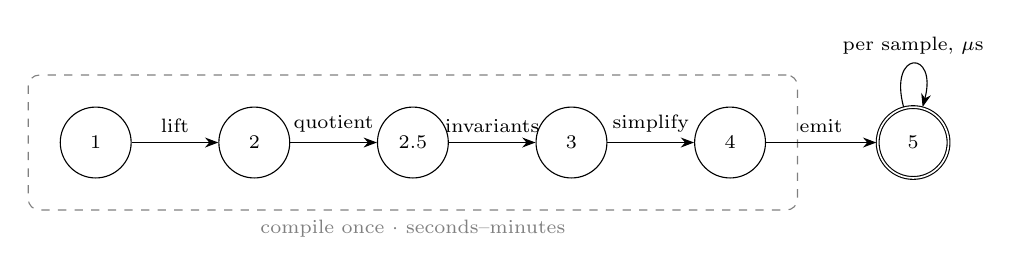
\begin{tikzpicture}[>=Stealth, font=\scriptsize, node distance=11mm,
    every state/.style={draw, circle, minimum size=9mm, inner sep=1pt}]
    \node[state] (s1) {1};
    \node[state, right=of s1]  (s2)  {2};
    \node[state, right=of s2]  (s25) {2.5};
    \node[state, right=of s25] (s3)  {3};
    \node[state, right=of s3]  (s4)  {4};
    \node[state, accepting, right=14mm of s4] (s5) {5};
    \draw[->] (s1)  -- node[above]{lift}        (s2);
    \draw[->] (s2)  -- node[above]{quotient}    (s25);
    \draw[->] (s25) -- node[above]{invariants}  (s3);
    \draw[->] (s3)  -- node[above]{simplify}    (s4);
    \draw[->] (s4)  -- node[above]{emit}         (s5);
    \draw[->] (s5)  to[loop above] node{per sample, $\mu$s} (s5);
    \begin{scope}[on background layer]
      \node[draw=gray, dashed, rounded corners, inner sep=4mm,
            fit=(s1)(s2)(s25)(s3)(s4),
            label=below:{\color{gray}compile once $\cdot$ seconds--minutes}] {};
    \end{scope}
  \end{tikzpicture}
  \end{center}
  \vspace{0.2em}
  \scriptsize
  \setlength{\tabcolsep}{5pt}
  \begin{center}
  \begin{tabular}{@{}lll@{}}
    \toprule
    Stage & Compiler analogue & What happens\\
    \midrule
    1 \;Symbolic lift        & parse / front-end        & instantiate templates $\to$ typed graph\\
    2 \;Symmetry quotient    & optimization pass        & rewrite collapsing equal work --- up to $48\times$ smaller\\
    2.5 Invariant synthesis  & semantic analysis        & a reduced basis fixed by the symmetry group\\
    3 \;Algebraic simplify   & classic IR optimization  & hash-consing, cross-formula CSE, tearing\\
    4 \;Lowering + adjoint   & codegen + reg.\ alloc.   & compression plans, synthesize adjoints, emit\\
    5 \;Runtime kernel       & the executable           & straight-line numeric code\\
    \bottomrule
  \end{tabular}
  \end{center}
  \note{Land the compiler framing. CSE, hash-consing, lowering are the same passes as in GCC/LLVM,
  running over physics expressions. Stage 2's symmetry pass is the one domain-specific
  optimization, buying a 48x constant factor for free.}
\end{frame}

\begin{frame}{Staging: pay the symbolic cost once}
  \framesubtitle{Compile once per problem; execute millions of times.}
  \begin{center}
  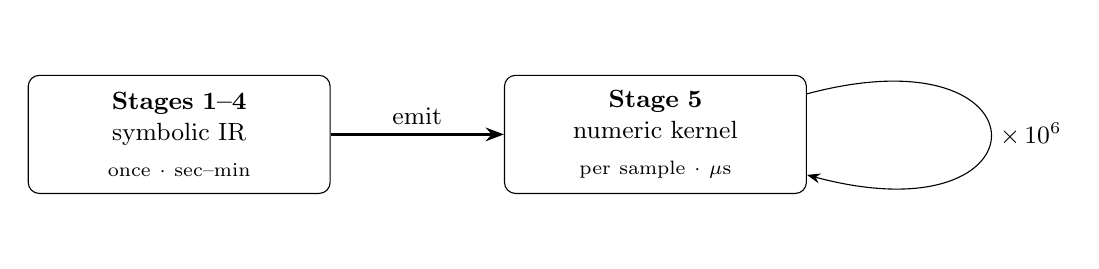
\begin{tikzpicture}[>=Stealth, font=\small, node distance=22mm]
    \node[draw, rounded corners, align=center, minimum height=15mm, text width=3.6cm] (c)
      {\textbf{Stages 1--4}\\ symbolic IR\\[2pt] {\scriptsize once $\cdot$ sec--min}};
    \node[draw, rounded corners, align=center, minimum height=15mm, text width=3.6cm,
          right=of c] (k)
      {\textbf{Stage 5}\\ numeric kernel\\[2pt] {\scriptsize per sample $\cdot$ $\mu$s}};
    \draw[->, thick] (c) -- node[above]{emit} (k);
    \draw[->] (k) to[loop right] node{$\times\,10^{6}$} (k);
  \end{tikzpicture}
  \end{center}
  \begin{itemize}\small
    \item The compile/runtime split is \textbf{multi-stage programming / partial evaluation}: all
      symbolic reasoning, symmetry reduction, and optimization is resolved at compile time
      \cz{\code{arch-07-pipeline} \S7.6}.
    \item This is \emph{why} checking is cheap: the system residualizes the physics once, then
      evaluates the residual forever.
  \end{itemize}
  \note{The microsecond cost on the cost-ladder slide is not luck, it is the payoff of staging ---
  partial evaluation / staged metaprogramming (Futamura) applied to physics.}
\end{frame}

% ===================================================================== Sec 4
\section{Structure and guarantees}

\begin{frame}{A type system over the quantities}
  \framesubtitle{Four orthogonal typeclasses give every quantity a type; the checkers dispatch on it.}
  \begin{columns}[T]
    \column{0.58\textwidth}
    \begin{itemize}\small
      \item Four Layer-0 typeclasses \cz{\code{arch-10-typeclasses}}:
        \code{Quantity} (value), \code{Sampleable} (shape), \code{HasAnalyticStructure} (law),
        \code{DiscreteStructure} (invariant).
      \item Cert checkers are ``generic functions over the typeclasses'' \cz{\S45--50} --- one
        checker per axis, reused across all physics.
      \item The same axes carry the algebra that makes composition lawful: an obligation-7
        \code{DiscreteStructure} morphism; \code{SymbolicTensorOps} as a colored operad
        \cz{\code{arch-20} \S98--103}; the Reynolds projector
        $P=\tfrac{1}{|G|}\sum_g \rho(g)$ onto the symmetry-fixed subspace, which provably
        preserves positive-semidefiniteness \cz{\code{arch-19}}.
    \end{itemize}
    \column{0.42\textwidth}
    \begin{center}
    \[
      \begin{tikzcd}[ampersand replacement=\&, row sep=large, column sep=large]
        V \arrow[r, "T"] \arrow[d, "\rho(g)"'] \& W \arrow[d, "\sigma(g)"]\\
        V \arrow[r, "T"'] \& W
      \end{tikzcd}
    \]
    {\footnotesize $T$ equivariant $\;\Leftrightarrow\;$ the square commutes.}
    \end{center}
  \end{columns}
  \note{State what each structure buys: typeclasses buy generic checkers (write once, dispatch
  everywhere); the operad buys lawful composition; the projector buys a by-construction guarantee
  (the assembled matrix stays positive-semidefinite). The payoff is the point.}
\end{frame}

\begin{frame}{Content addressing}
  \framesubtitle{Every object is named by the hash of its content.}
  \begin{center}\small
    \code{Address[D] = Hash(domain\_sep, schema\_version, canonical\_bytes)}
    \cz{\code{arch-20-representations} \S20.4}
  \end{center}
  \vspace{0.4em}
  \begin{itemize}
    \item \textbf{Memoization \& dedup} --- identical sub-expressions collapse to one node
      (hash-consing).
    \item \textbf{Tamper-evidence} --- changing any payload changes its hash and trips the freeze
      comparison \cz{\code{arch-12-cert} \S155--160}.
    \item \textbf{Structural sharing} --- the whole IR is a Merkle DAG, like Git commits or a
      build cache.
  \end{itemize}
  \note{The most relatable analogy: a content hash as a name, applied to physics expressions. It is
  where the reproducibility and caching guarantees come from.}
\end{frame}

\begin{frame}{Differentiation as a first-class output}
  \framesubtitle{The oracle returns gradients, not just scores --- cheaply.}
  \begin{itemize}
    \item Stage 5 emits \textbf{gradients} $\partial R/\partial\hat{x}$ alongside the residuals
      --- reverse-mode AD built into the kernel.
    \item The \textbf{implicit-function-theorem adjoint} makes the gradient of a fixed-point solve
      cost ``one extra linear solve, independent of forward iteration count''
      \cz{\code{arch-07-pipeline} \S133--137} --- the verify-cheap asymmetry, now for derivatives.
    \item The bridge to the learned model is a typed \textbf{calling convention}: the oracle
      returns $\partial R/\partial\hat{x}$; the consumer ``brings its own backward'' to chain
      $\partial\hat{x}/\partial\theta$ \cz{\code{arch-16-pino-bridge}}. Three exports ---
      \code{Generate} / \code{Validate} / \code{Import} --- form the interface.
  \end{itemize}
  \note{Even differentiation obeys verify < solve --- the adjoint replaces an unrolled iteration
  with a single linear solve. Bring-your-own-backward is the clean seam; keep the learner offstage.}
\end{frame}

\begin{frame}{Well-formedness, checked by the compiler}
  \framesubtitle{Ill-formed physics is rejected mechanically, before it ever runs.}
  \begin{itemize}
    \item Registration is a \textbf{decidable gate}: every applicability predicate is
      ``first-order decidable --- finite case analysis on typeclass tags, not numeric thresholds''
      \cz{\code{impl-04-formulas}}.
    \item The \textbf{adjoint gate} fails the build when a derived gradient disagrees with a
      finite-difference check beyond $\tau_{\mathrm{adj}}$ \cz{\code{impl-07} \S7.5}.
    \item Compose-time \textbf{refusals} reject inconsistent compositions by tag comparison --- an
      unprovenanced coefficient, or a double-counted temperature path \cz{\code{arch-12} \S12.0.3}.
    \item The 13-phase build sequence \cz{\code{impl-10-build-sequence}} is the state machine that
      enforces all of it.
  \end{itemize}
  \note{Correctness is a property the compiler checks, so a registered composition is well-formed by
  construction --- the same guarantee a strongly-typed language gives, caught at build time.}
\end{frame}

\begin{frame}{Where each guarantee comes from}
  \framesubtitle{Each property the system promises traces to one mechanism.}
  \setlength{\tabcolsep}{8pt}
  \renewcommand{\arraystretch}{1.25}
  \begin{center}
  \begin{tabular}{@{}ll@{}}
    \toprule
    Guarantee & Comes from\\
    \midrule
    \textbf{Speed} & staged compilation $+$ the verify $<$ solve asymmetry\\
    \textbf{Exhaustiveness} & a closed grammar $+$ decidable applicability\\
    \textbf{Trust} & checkable certificates $+$ content-addressed tamper-evidence\\
    \textbf{Composability} & an AST with a type system\\
    \textbf{Gradients} & first-class AD $+$ implicit-function adjoints\\
    \bottomrule
  \end{tabular}
  \end{center}
  \vspace{1em}
  \centering\itshape The physics is the domain; the machinery above is what makes it a system.
  \note{Point at each row: the promise on the left, the one mechanism that delivers it on the right.
  End on the closing line and stop; let it sit.}
\end{frame}

% ===================================================================== Backup
\appendix

\begin{frame}{Backup --- Q\&A reserve}
  Held in reserve for domain-expert questions:
  \begin{itemize}\small
    \item The full closed-vocabulary tables (12 methods, 20 templates, 125 formulas, 11 bundles).
    \item The 19 residual categories \cz{\code{arch-11-residuals} \S11.1}: 9 equation-of-motion,
      3 structural, 5 algebraic-identity, 2 constraint.
    \item The 10 cert obligations in full \cz{\code{arch-12-cert} \S24--40}.
    \item The tier/cost/cadence table with per-tier examples \cz{\code{impl-07} \S175--191}.
    \item The error model: a per-residual budget composed from input $\sigma$, model-form error,
      compression truncation, dressing staleness, and coefficient-provenance $\sigma$
      \cz{\code{arch-11-residuals} \S11.7}.
  \end{itemize}
\end{frame}

\begin{frame}{Appendix --- concept to where it lives}
  \scriptsize
  \setlength{\tabcolsep}{5pt}
  \renewcommand{\arraystretch}{1.15}
  \begin{tabular}{@{}lll@{}}
    \toprule
    Concept & In \code{/physics} & Source\\
    \midrule
    NP certificate / verify $<$ solve     & the cert + the scoring principle        & \code{arch-12, arch-01, arch-21}\\
    Complexity tiers of checking          & cadence T0--T3                          & \code{impl-07} \S175--191\\
    Formal language / closed grammar      & the vocabularies                        & \code{arch-09}\\
    AST + typing rules                    & PhysicsGraph, 3 node kinds              & \code{arch-06}\\
    Compiler passes (CSE, lowering)       & Stages 1--5                             & \code{arch-07}\\
    Partial evaluation / staging          & compile-once / run-per-sample           & \code{arch-07} \S7.6\\
    Type system / typeclass dispatch      & 4 Layer-0 typeclasses                   & \code{arch-10, arch-12}\\
    Category theory (operad, morphism)    & SymbolicTensorOps, obligation 7         & \code{arch-20, arch-19}\\
    Lattice theory                        & verdict semilattice meet                & \code{impl-07} \S56--60\\
    Merkle DAG / content addressing       & \code{Address}, hash-consing            & \code{arch-20} \S20.4\\
    Reverse-mode AD / implicit adjoint    & gradient exports                        & \code{arch-07} \S133--137, \code{arch-16}\\
    Decidability / build automaton        & applicability gate, refusals, 13-phase  & \code{impl-04, impl-10, arch-12}\\
    \bottomrule
  \end{tabular}
\end{frame}

\end{document}
